
\par $S_{cheio_{fome}} = [2,2]$

\vskip 0.3in
\par $S_{alternativa^{+}} = [1,1]$ \qquad $S_{alternativa^{-}} = [1,1]$
\par $H(S_{alternativa^{+}}) = -\frac{1}{2} \log_2 \frac{1}{2}- \frac{1}{2} \log_2 \frac{1}{2} = 1.000$
\par $H(S_{alternativa^{-}}) = -\frac{1}{2} \log_2 \frac{1}{2}- \frac{1}{2} \log_2 \frac{1}{2} = 1.000$
\par $Ganho(S, S_{alternativa}) = 1.000-\frac{2}{4} * 1.000-\frac{2}{4} * 1.000 = 0.000$

\vskip 0.3in
\par $S_{bar^{+}} = [1,1]$ \qquad $S_{bar^{-}} = [1,1]$
\par $H(S_{bar^{+}}) = -\frac{1}{2} \log_2 \frac{1}{2}- \frac{1}{2} \log_2 \frac{1}{2} = 1.000$
\par $H(S_{bar^{-}}) = -\frac{1}{2} \log_2 \frac{1}{2}- \frac{1}{2} \log_2 \frac{1}{2} = 1.000$
\par $Ganho(S, S_{bar}) = 1.000-\frac{2}{4} * 1.000-\frac{2}{4} * 1.000 = 0.000$

\vskip 0.3in
\par $S_{fimSemana^{+}} = [2,1]$ \qquad $S_{fimSemana^{-}} = [0,1]$
\par $H(S_{fimSemana^{+}}) = -\frac{2}{3} \log_2 \frac{2}{3}- \frac{1}{3} \log_2 \frac{1}{3} = 0.918$
\par $H(S_{fimSemana^{-}}) = -\frac{0}{1} \log_2 \frac{0}{1}- \frac{1}{1} \log_2 \frac{1}{1} = 0.000$
\par $Ganho(S, S_{fimSemana}) = 1.000-\frac{3}{4} * 0.918-\frac{1}{4} * 0.000 = 0.311$

\vskip 0.3in
\par $S_{preço^{\$}} = [1,0]$ \qquad $S_{preço^{\$\$\$}} = [2,1]$
\par $H(S_{preço^{\$}}) = -\frac{1}{1} \log_2 \frac{1}{1}- \frac{0}{1} \log_2 \frac{0}{1} = 0.000$
\par $H(S_{preço^{\$\$\$}}) = -\frac{2}{3} \log_2 \frac{2}{3}- \frac{1}{3} \log_2 \frac{1}{3} = 0.918$
\par $Ganho(S, S_{preço}) = 1.000-\frac{1}{4} * 0.000-\frac{3}{4} * 0.918 = 0.311$

\vskip 0.3in
\par $S_{chuva^{+}} = [1,0]$ \qquad $S_{chuva^{-}} = [1,2]$
\par $H(S_{chuva^{+}}) = -\frac{1}{1} \log_2 \frac{1}{1}- \frac{0}{1} \log_2 \frac{0}{1} = 0.000$
\par $H(S_{chuva^{-}}) = -\frac{1}{3} \log_2 \frac{1}{3}- \frac{2}{3} \log_2 \frac{2}{3} = 0.918$
\par $Ganho(S, S_{chuva}) = 1.000-\frac{1}{4} * 0.000-\frac{3}{4} * 0.918 = 0.311$

\vskip 0.3in
\par $S_{reserva^{+}} = [0,1]$ \qquad $S_{reserva^{-}} = [2,1]$
\par $H(S_{reserva^{+}}) = -\frac{0}{1} \log_2 \frac{0}{1}- \frac{1}{1} \log_2 \frac{1}{1} = 0.000$
\par $H(S_{reserva^{-}}) = -\frac{2}{3} \log_2 \frac{2}{3}- \frac{1}{3} \log_2 \frac{1}{3} = 0.918$
\par $Ganho(S, S_{reserva}) = 1.000-\frac{1}{4} * 0.000-\frac{3}{4} * 0.918 = 0.311$

\vskip 0.3in
\par $S_{tipo^{Tailandês}} = [1,1]$ \qquad $S_{tipo^{Italiano}} = [0,1]$\par $S_{tipo^{Hamburger}} = [1,0]$
\par $H(S_{tipo^{Tailandês}}) = -\frac{1}{2} \log_2 \frac{1}{2}- \frac{1}{2} \log_2 \frac{1}{2} = 1.000$
\par $H(S_{tipo^{Italiano}}) = -\frac{0}{1} \log_2 \frac{0}{1}- \frac{1}{1} \log_2 \frac{1}{1} = 0.000$
\par $H(S_{tipo^{Hamburger}}) = -\frac{1}{1} \log_2 \frac{1}{1}- \frac{0}{1} \log_2 \frac{0}{1} = 0.000$
\par $Ganho(S, S_{tipo}) = 1.000-\frac{2}{4} * 1.000-\frac{1}{4} * 0.000-\frac{1}{4} * 0.000 = 0.500$

\vskip 0.3in
\par $S_{tempoEspera^{10-30}} = [1,1]$ \qquad $S_{tempoEspera^{30-60}} = [1,1]$
\par $H(S_{tempoEspera^{10-30}}) = -\frac{1}{2} \log_2 \frac{1}{2}- \frac{1}{2} \log_2 \frac{1}{2} = 1.000$
\par $H(S_{tempoEspera^{30-60}}) = -\frac{1}{2} \log_2 \frac{1}{2}- \frac{1}{2} \log_2 \frac{1}{2} = 1.000$
\par $Ganho(S, S_{tempoEspera}) = 1.000-\frac{2}{4} * 1.000-\frac{2}{4} * 1.000 = 0.000$

\vskip 0.4in
\hfil
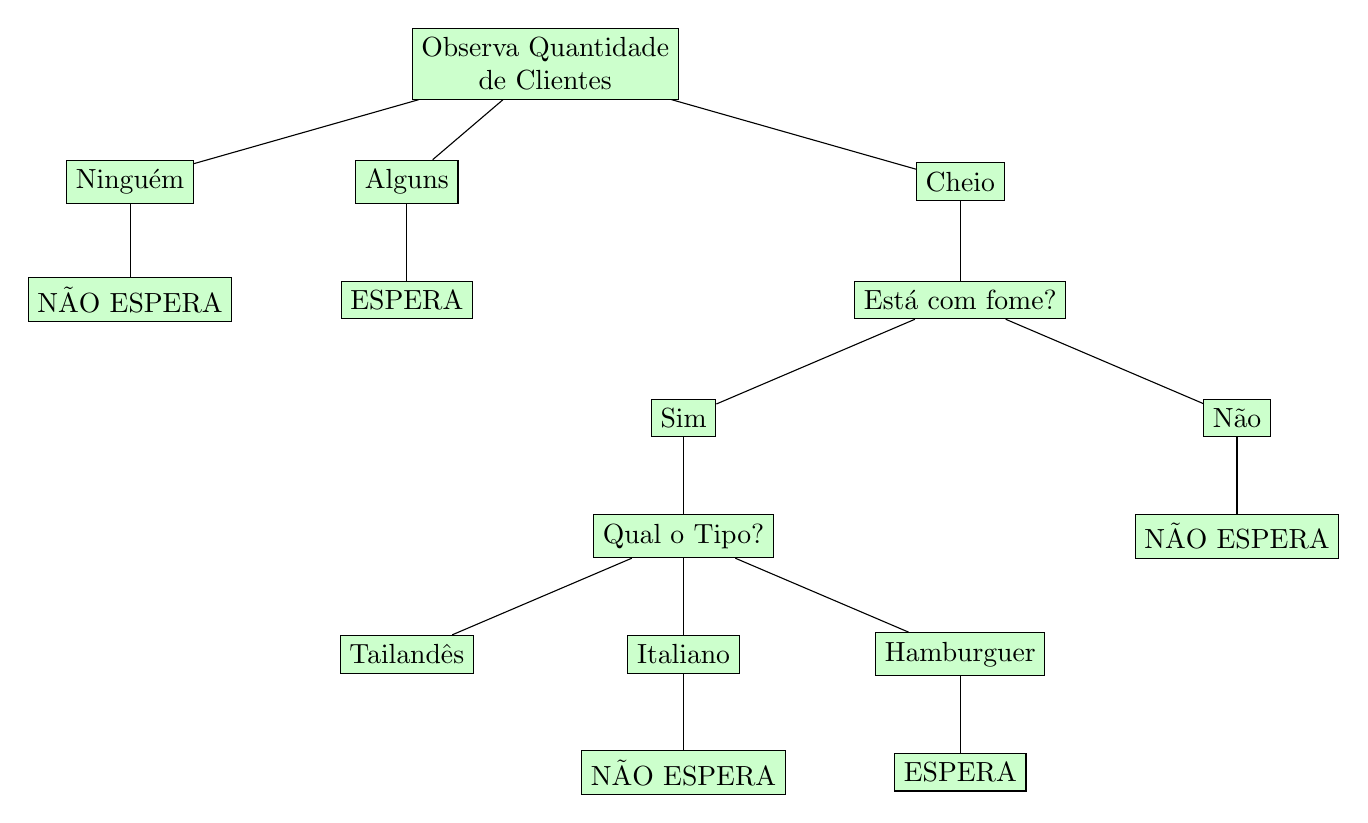
\begin{tikzpicture}[sibling distance=10em,
    every node/.style = {shape=rectangle, 
      draw, align=center,
      top color=green!20, bottom color=green!20}]]
    \node {Observa Quantidade \\ de Clientes}
        child { node {Ninguém} child { node {NÃO ESPERA}  } }
        child { node {Alguns} child { node {ESPERA}  } }
        child [missing]
        child { node {Cheio} child { 
            node {Está com fome?} 
            child { node {Sim} child { node {Qual o Tipo?} 
                 child { node {Tailandês} }   
                 child { node {Italiano}  child { node {NÃO ESPERA}  }  } 
                 child { node {Hamburguer} child { node {ESPERA}  } } 
            }   }
            child [missing]
            child { node {Não} child { node {NÃO ESPERA}  }  }
            }
        };
  \end{tikzpicture}